%------------------------------------------------------------------------------
%	CAPITOLO 16
%------------------------------------------------------------------------------

\chapter{Come si può cambiare bandiera}
I più arrabbiati papalini del paese erano \index[Personaggi]{Bagnara Giovanni}Bagnara, del quale ci siamo occupati, il fabbro \index[Personaggi]{Cappelli Paolo}Paolo Cappelli della \index[Luoghi]{Tosca}Tosca ed il vecchio \index[Personaggi]{Bartolotti Francesco}Bartolotti\footnote{\textbf{Bartolotti Francesco} fu un consigliere comunale insieme a \textbf{Giovanni Bagnara} attorno al 1855}, che abitava al \index[Luoghi]{Cortilazzo}Cortilazzo, poco prima della \index[Luoghi]{Tosca}Tosca. Passando per la strada gli austriaci, in parecchi ebbero necessità urgente di soddisfare certe occorrenze corporali e si rifugiavano nel cortile del \index[Personaggi]{Bartolotti Francesco}Bartolotti.\\
\indent Non ci volle altro! Prima così fermo nelle sue idee papaline, austriacanti reazionare e resistenti alle minacce liberali... il vecchio \index[Personaggi]{Bartolotti Francesco}Bartolotti disertò, per questa offesa al suo suolo, il campo e passò nel campo liberale in armi e bagaglio!\\
\indent I suoi compagni \index[Personaggi]{Bagnara Giovanni}Bagnara e \index[Personaggi]{Cappelli Paolo}Cappelli non gliela perdonarono e specialmente quest'ultimo, cliente e amico del magnano\footnote{Artigiano che esegue minuti lavori in ferro} \index[Personaggi]{Gregori Giovacchino}Giovacchino\footnote{\textbf{Gregori Giovacchino}, uno dei fratelli di Attilio Gregori\index[Personaggi]{Gregori Attilio}, il nonno di Attilio che è attualmente proprietario della ferramenta Gregori di Alfonsine. Giovacchino aprì una ferramenta a \index[Luoghi]{Lavezzola}Lavezzola. La famiglia Gregori è originaria del Trentino-Alto Adige e ad Alfonsine vengono chiamati `Magnên'.} (trentino di nascita) quando passava per andare o tornare a piedi per recarsi nel Trentino lo chiamava e gli diceva:\\
\indent <<Juvachìn a iei i fradèl a \index[Luoghi]{Pontelagoscuro}Pont Legscur\footnote{<<Giovacchino, ci sono i fratelli austriaci a Pontelagoscuro?>> - Pontelagoscuro è una frazione del comune di Ferrara}?>>\\
\indent Juvachìn rispondeva: <<Oh, sè\footnote{<<Oh, si>>}>>.\\
\indent \index[Personaggi]{Cappelli Paolo}Cappelli: <<Alora disìi cossa chi fa chin ven in qua ad amazé tot sti vigliac d'Italièn\footnote{<<Allora dite(chiedete) loro che cosa fanno che non vengono qua ad ammazzare questi vigliacchi d'Italiani>>}>>.\\
\indent Poi grattava e si calcava in testa la papalina, riprendeva il lavoro per consolare la sua ira.

 \begin{figure}[htb]
    \centering
    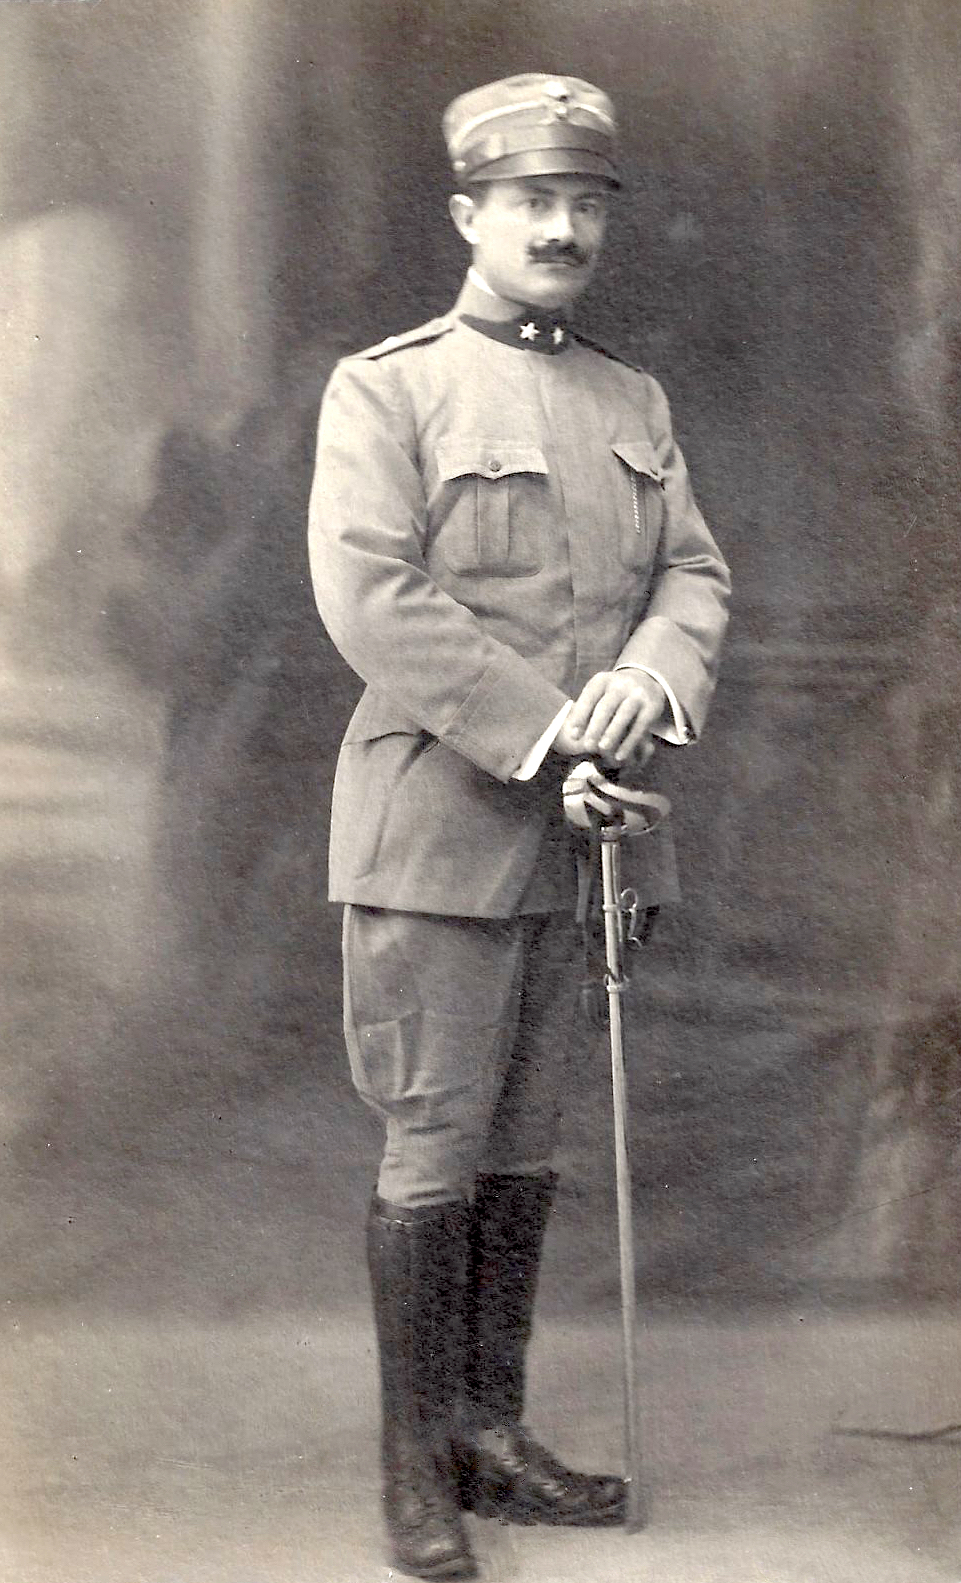
\includegraphics[width=0.75\textwidth]{mingazzisoldato}
    \caption[Stefano Mingazzi in divisa militare]{Stefano Mingazzi\index[Personaggi]{Mingazzi Stefano}, in veste da Tenente ufficiale del Regio Esercito.\label{fig:mingazzisoldato}}
    \vspace{-0.8cm}
\end{figure}